%!TEX root = ../main.tex

\section{Border marking, labeling and routing}
\label{sec:border_marking}

A depthmap is a 2D parameterization of a 3D scene visualized from a specific point of view. From this representation it is possible to obtain a point cloud representing the samples acquired from this specific point of view (Figure \ref{fig:depthmap_point_cloud}(b)).

This link between depth values and 3D coordinates motivated us using depthmaps as a parameterization domain to apply algorithm on point clouds, considering the implicit connectivity between pixels to do local computations requesting the consideration of neighboring points.

If most of the time it is correct to consider that neighboring pixels in a depthmap are also neighbors on the surface (with respect to the sampling density of the acquisition), it is not the case along depth discontinuities (Fig \ref{fig:depth_discontinuity}).
Since an acquisition is done from a specific position and orientation, it can only represent visible points from that specific point of view. 
Thus many surface areas can be occluded, and different surface areas could be considered "touching" each other in the depthmap, even if they are far on the surface.

To avoid this, we present a method to mark the borders, identify each of them uniquely and store the path from the beginning until the end of each border.

Many methods have been developed to detect borders and to segmentate however those techniques only seek to separate different areas of the image, or image parts where specific processing should be applied.
In our case, we want not only to detect borders, but also to store the path that each border follows.

\begin{figure}
\centering
\scalebox{0.05}{
\begin{tikzpicture}[spy using outlines={circle, red, magnification=10, size=50cm, connect spies}]
\node {\pgfimage{Images/DepthMap-Garuda}};
\spy on (5,-1) in node [left] at (100,0);
\end{tikzpicture}
\begin{tikzpicture}[spy using outlines={circle, red, magnification=10, size=50cm, connect spies}]
\node {\pgfimage{Images/Borders-Garuda}};
\spy on (5,-1) in node [left] at (100,0);
\end{tikzpicture}
}
\caption{High depth variation between neighboring pixels that do not belong to neighboring surface areas (left), and the detected associated borders (right).}
\label{fig:depth_discontinuity}
\end{figure}

\subsection{Border marking}
First, we mark all the pixels of the depthmap that do not fulfill a local depth-discontinuity condition. We consider a depth-discontinuity as being an important change of depth in at least one direction (horizontal, vertical or diagonal).

During that step, we are defining how points would be triangulated if a mesh was going to be constructed between neighboring pixels over the whole depthmap. 
For this, we consider an arbitrary connectivity pattern, connecting one pixel to 6 of its neighbors (Figure \ref{fig:pixel_neighborhood}). 

\begin{figure}[ht]
\centering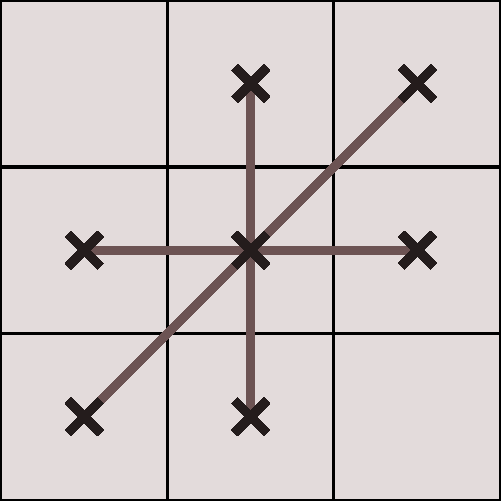
\includegraphics[scale=0.4]{PixelNeighborhood}
\caption{The 6-neighborhood considered around each pixel}
\label{fig:pixel_neighborhood}
\end{figure}

For each pixel $p$, we search to know if there a high intensity variation with respect to each of his neighbors. If this is the case, it means that the two pixels do not belong the same surface area, and then need to be separated for the further processings.
But instead of using a fixed threshold over the entire depthmap, we consider a variable parameter, which value will vary with respect to the distance from the camera.
This comes from the fact that 3D scanners acquire a higher density of points when objects are closer than when they are further. 
Thus by weighting a chosen threshold with pixel intensities, we are able to have a threshold that will vary with respect to the depth, i.e it will be smaller for high density areas, and bigger for low density areas.

To understand how the threshold is weighted, it important to remember that the distance between two specific points increases when their depth increases.
However it doesn't 

\subsection{Border labeling and routing}
Now that borders have been indentified, we need to label them in order to be able to consider them independently. 

Each border is represented as a list, characterizing the path from pixel to pixel, from the beginning until the end of the border.

We decide to use a region-growing process. 
Starting from a pixel that has been marked as a border, we search the next pixel defining the same border. 
This is equivalent as searching the next vertex along the border of the triangulation, by considering that faces are oriented.
When this pixel has been found, it is added to the current border list, and being processed, to find the next pixel of the border after him.
When there is no more pixel than can be added to the current border, the border is considered as completed.

At the initialization, every pixel marked as a border is added to a list. Until this list is not empty, the first pixel is treated and removed from the list. 
If the pixel isn't already labeled it is used as the starting pixel of a new border, following the steps.
If the pixel has already been labeled, then it is ignored, and the next one is considered instead. 

\begin{figure}[ht]
\centering
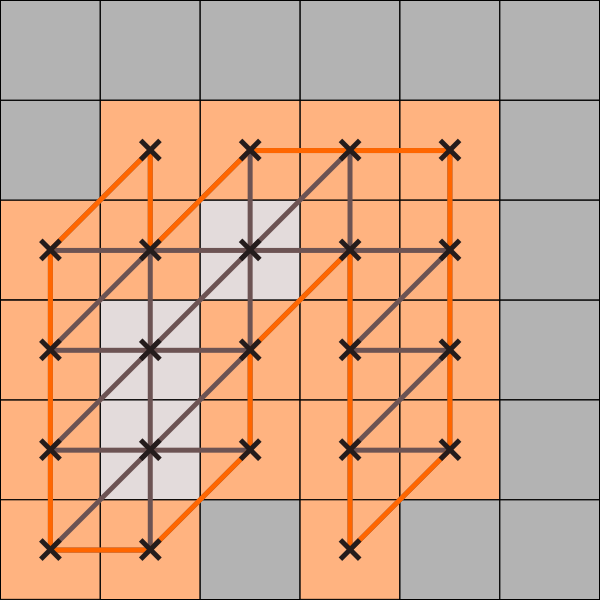
\includegraphics[scale=0.3]{PixelTriangulationBorder}
\caption{Implicit triangulation of a depthmap constructed when finding the border pixels. Darker pixels represent background, lighter and orange represent the object, and orange pixels alone represent the pixels marked as "borders".
Edges in orange are the edges defining the border of the triangulation.}
\label{fig:border_triangulation}
\end{figure}